\section{Baseline results}

\textbf{Baseline.} The proposal's baseline was a box prompt, GrabCut \cite{grabcut} initialized
from that rectangle, and a translation-only tracker. It finds Shi--Tomasi corners \cite{shitomasi},
follows them with pyramidal Lucas--Kanade flow \cite{lk}, and shifts the mask by their median
displacement. Iteration~1 in the proposal swapped the box for a freehand outline. Before adding
anything new, we wanted a benchmark we could rerun after every change.

\textbf{Evaluation.} The synthetic benchmark has four 90-frame clips that each test one thing.
There's plain translation, a scale change where the object shrinks to 45\% of its starting size, an
occlusion where it passes completely behind a pillar, and a scene cut at frame 45. We simulate the
user's prompt from the first-frame ground truth with 5, 9, and 13 pixels of slack. We also test on
real video now, using 12 objects from 8 DAVIS 2017 \cite{davis} sequences and 6 hand-labeled frames
of our 150-frame crosswalk clip. We report mask IoU before dilation, plus the uncovered target
share (the proposal's leak rate), which is the fraction of visible target pixels still exposed after
the $9{\times}9$ safety dilation. Later ground-truth masks never get fed into tracking.

\textbf{Why the baseline numbers moved.} We lost the script behind the proposal's table, so we
rebuilt the synthetic clips from its description. The new numbers are close but not identical
(Table~\ref{tab:baseline}). Both versions agree on the important part. Moving is easy, and
shrinking, occlusion, and cuts all break the tracker. From here on, ``original'' means the rebuilt
outline baseline, since the outline is our default selection.

\begin{table}[h]
\centering\small
\begin{tabular}{lcccc}
\toprule
IoU & Translation & Scale & Occlusion & Scene cut \\
\midrule
Proposal, box baseline (original script, mean of 3 slacks) & 0.85 & 0.41 & 0.37 & 0.43 \\
Rebuilt, box baseline (5-px slack) & 0.913 & 0.469 & 0.343 & 0.457 \\
Rebuilt, outline baseline (5-px slack) & 0.881 & 0.456 & 0.317 & 0.440 \\
\bottomrule
\end{tabular}
\caption{The proposal's baseline next to the rebuilt benchmark.}
\label{tab:baseline}
\end{table}

\begin{figure}[h]
\centering
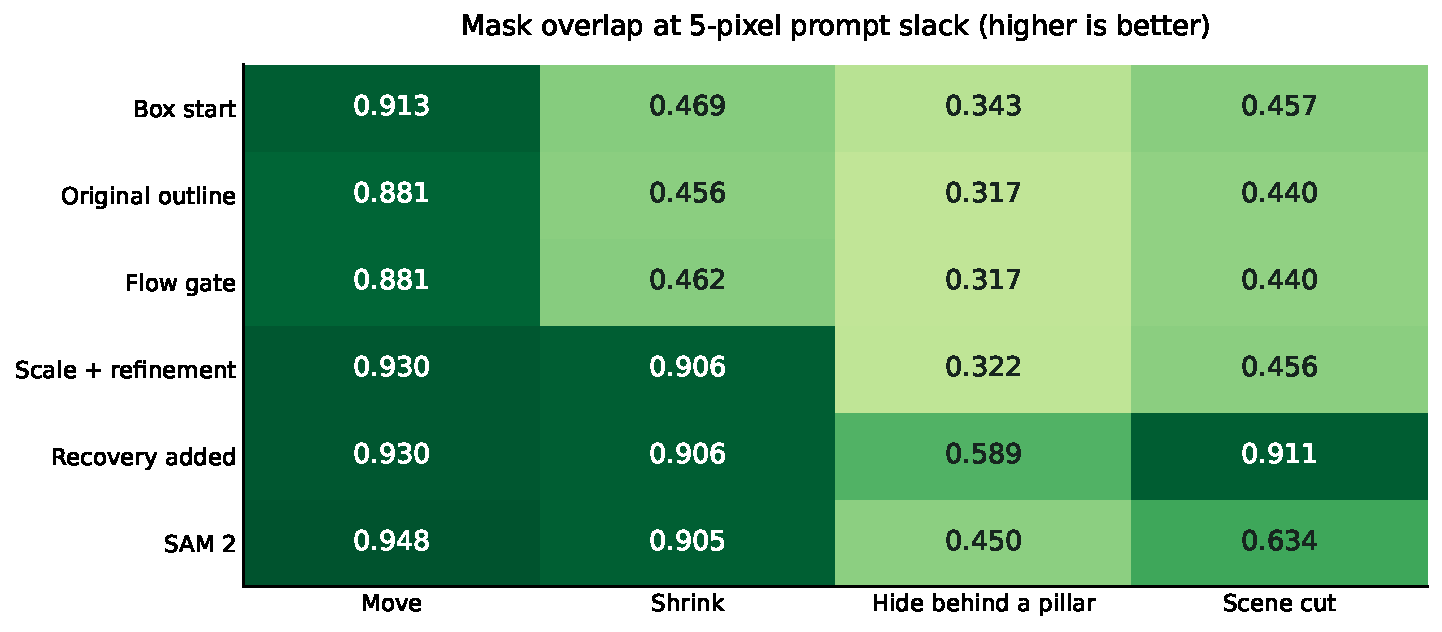
\includegraphics[width=\linewidth]{figures/iterations.pdf}
\caption{One slice of the 72-run synthetic comparison (6 variants $\times$ 4 clips $\times$ 3 prompt
sizes) at 5-pixel slack. Darker means better overlap. The flow gate is the proposal's
forward-backward check \cite{fb}, brought back for comparison.}
\label{fig:variants}
\end{figure}

Figure~\ref{fig:variants} shows where the baseline breaks. Movement was easy, and the outline
tracker already hit 0.881 IoU. Scale was the first real problem. IoU fell to 0.456 when the target
shrank, because shifting a mask never makes it smaller. The flow gate didn't help with occlusion
(0.317) or cuts (0.440). Like we found in the proposal, noticing a bad frame doesn't find the
target again. So the plan was to fix the motion model first and then add a way to search for a lost
target.

\section{Iteration results}

\subsection{Iteration 2: scale-aware motion and appearance recovery}

\textbf{Change A, scale-aware motion.} Instead of using the median point displacement, we check
the flow forward and backward, fit a similarity transform (translation, rotation, and scale) with
RANSAC \cite{ransac}, warp the mask, and run GrabCut on it again. RANSAC throws out points that move
inconsistently, like ones that slid onto the background, and re-segmenting keeps the edges from
drifting. This fixed the scale failure, with shrinking-clip IoU going from 0.456 to 0.906
(Table~\ref{tab:iter2}). It did nothing for occlusion (0.317 to 0.322), which made sense to us.
While the target is behind the pillar there's nothing to track, and a better motion model can't
change that.

\textbf{Change B, searching when motion is unreliable.} On the first frame we save the target's
color histogram and an appearance template. When tracking gets uncertain, the tracker stops trusting
the last mask and searches the frame for the template at several scales. If two spots match about
equally well, we reject the match instead of guessing. A histogram-based scene-cut check triggers
the same search.

\begin{table}[h]
\centering\small
\begin{tabular}{lccc}
\toprule
Test and metric & Original & Scale fix & + Recovery \\
\midrule
Scale, IoU & 0.456 & 0.906 & 0.906 \\
Occlusion, IoU & 0.317 & 0.322 & 0.589 \\
Occlusion, uncovered target & 50.0\% & 50.0\% & 18.3\% \\
Scene cut, IoU & 0.440 & 0.456 & 0.911 \\
Scene cut, uncovered target & 49.8\% & 47.4\% & 0.0\% \\
\bottomrule
\end{tabular}
\caption{Iteration 2 on the synthetic clips at 5-pixel prompt slack.}
\label{tab:iter2}
\end{table}

\textbf{Real-video result.} Testing on real video changed the picture (Table~\ref{tab:iter2real}).
Iteration~2 was a big win on the synthetic clips and barely moved anything on real footage. On the
crosswalk it was actually worse than the original. The per-frame log shows why
(Table~\ref{tab:crosswalk-frames}). The mask didn't drift onto other people. By frame 30 it covered
almost nothing outside the target, so it was only sitting on part of her, and by frame 60 it was
leaving 72\% of her uncovered. At frame 90 the tracker marked her as lost, and recovery never found
her again for the rest of the clip. The original tracker never gives up, so it kept a partial
overlap for longer, and that's why it scored better on average. We think the frozen template is the
problem. The synthetic target is a rigid, textured shape that looks the same in every frame, which
is exactly what a template is good at. A real pedestrian changes pose every step and gets smaller
as she walks away, so the first-frame template stops matching her. The uncertainty checks also fired
on 53\% of crosswalk frames. The takeaway for us was that we'd tuned the tracker to our own test
clips.

\begin{table}[h]
\centering\small
\begin{tabular}{lcccccc}
\toprule
Crosswalk frame & 0 & 30 & 60 & 90 & 120 & 149 \\
\midrule
Original, IoU & 0.898 & 0.597 & 0.481 & 0.353 & 0.085 & 0.000 \\
Iteration 2, IoU & 0.898 & 0.382 & 0.199 & 0.000 & 0.000 & 0.000 \\
Iteration 2, uncovered target & 0\% & 54\% & 72\% & 100\% & 100\% & 100\% \\
Iteration 2, confidence & 1.00 & 0.71 & 0.73 & lost & lost & lost \\
\bottomrule
\end{tabular}
\caption{The six labeled crosswalk frames. Iteration 2's mask shrinks onto part of the target and
then the tracker loses her for good at frame 90.}
\label{tab:crosswalk-frames}
\end{table}

\begin{table}[h]
\centering\small
\begin{tabular}{lcc}
\toprule
Mean IoU & Original & Iteration 2 \\
\midrule
Synthetic, all three prompt sizes & 0.495 & 0.812 \\
DAVIS subset & 0.298 & 0.310 \\
Crosswalk & 0.402 & 0.246 \\
\bottomrule
\end{tabular}
\caption{Iteration 2 on synthetic and real video.}
\label{tab:iter2real}
\end{table}

\subsection{Iteration 3: SAM 2}

\textbf{Change.} We replaced stages 2 and 3 with the official pretrained SAM~2.1 Tiny video model
\cite{sam2}, which carries a prompted mask through the video using a memory of past frames. Our
code still handles prompts, target ids, corrections, covering, and review. To fit on the 6\,GB
laptop GPU, we keep frames and model state in CPU memory.

\textbf{Result.} SAM~2 was way better on real video (Table~\ref{tab:sam2}, Figure~\ref{fig:sam2}).
On DAVIS, IoU went from 0.310 to 0.835 and the uncovered share dropped from 47.67\% to 2.21\%, at
about the same speed.

\begin{table}[h]
\centering\small
\begin{tabular}{lcc}
\toprule
DAVIS subset & Iteration 2 & SAM 2 \\
\midrule
Mean IoU & 0.310 & 0.835 \\
Mean uncovered target & 47.67\% & 2.21\% \\
Median propagation speed & 7.2 fps & 6.3 fps \\
\bottomrule
\end{tabular}
\caption{Iteration 3 on DAVIS, run on an RTX 4050 Laptop GPU. Timing leaves out model loading and
video encoding. These are single runs and not a controlled speed study, and both are below real
time (30 fps).}
\label{tab:sam2}
\end{table}

\begin{figure}[h]
\centering
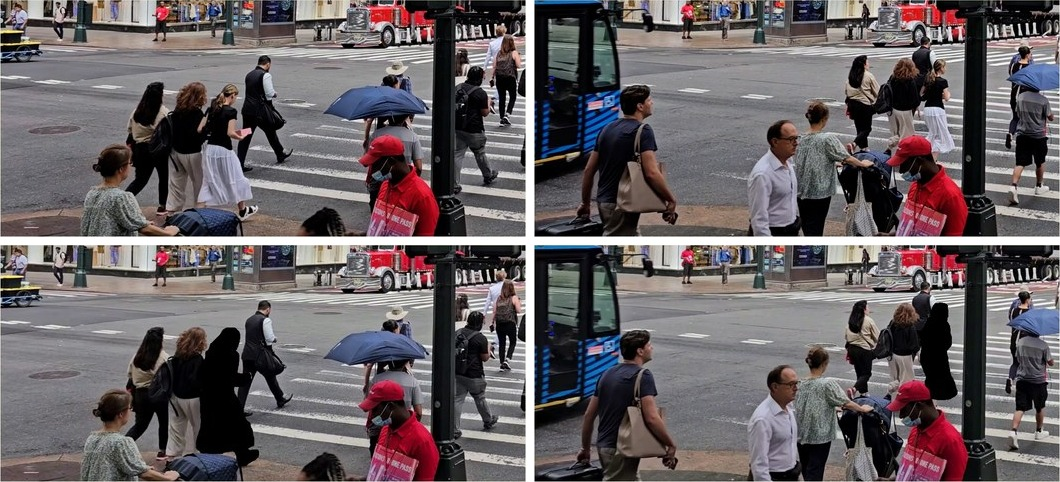
\includegraphics[width=0.88\linewidth]{figures/crosswalk-sam2.jpg}
\caption{The proposal's crosswalk clip with SAM 2. The top row is the input and the bottom row is
the output, with the woman in the white skirt covered. In the proposal, the classical tracker's
mask had slid onto bystanders by these frames (crosswalk IoU 0.779 vs.\ 0.402).}
\label{fig:sam2}
\end{figure}

SAM~2 wasn't the best everywhere, though. On the synthetic pillar clip it left 48.9\% of the target
uncovered, worse than Iteration~2's 18.3\%. On DAVIS \texttt{bmx-trees/1} its IoU was only 0.443,
because SAM~2 keeps a confident mask on part of the rider while the trees cover the rest. We come
back to the pillar failure in Iteration~4.

\textbf{Side experiment with ResNet features.} We also tried swapping Iteration~2's color and
template search for frozen ImageNet ResNet-18 features \cite{resnet}, keeping motion and refinement
the same. We expected learned features to handle pose changes better, but they didn't
(Figure~\ref{fig:resnet}). DAVIS IoU fell from 0.310 to 0.284 and synthetic IoU from 0.812 to 0.769.
Crosswalk IoU went up a little (0.246 to 0.263), but both were still far behind SAM~2's 0.779 there.
Our best guess is that we were still matching a fixed spatial feature map from the first frame, so
the features carried over the original pose and shape. We didn't fine-tune anything on our clips,
and we left this option in as an experiment only.

\begin{figure}[h]
\centering
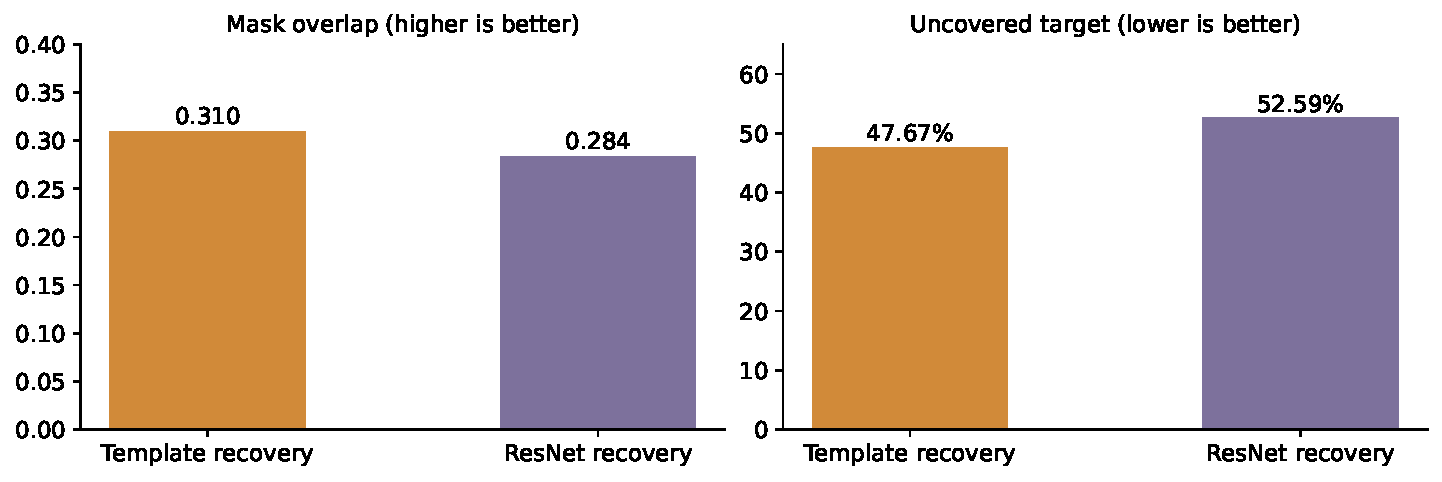
\includegraphics[width=0.9\linewidth]{figures/recovery.pdf}
\caption{Classical vs.\ ResNet recovery on DAVIS (12 objects).}
\label{fig:resnet}
\end{figure}

\textbf{Covering the whole frame can hide a bad tracker.} Our safety policy covers the entire frame
whenever the tracker is uncertain. For Iteration~2 on DAVIS, that brought the uncovered share down
from 47.67\% to 9.29\%, but the extra frame area covered went from 4.1\% to 58.3\%. It's a fine
fallback, but it makes Iteration~2 look better than it really is. Since then we always report extra
coverage alongside misses.

\subsection{Iteration 4: appearance recovery inside SAM 2}

\textbf{What went wrong in Iteration 3.} The per-frame log on the pillar clip showed SAM~2 tracking
the target well up to the pillar and correctly marking it hidden for frames 41--48. After that it
never picked the target back up, and every frame from 49 to 89 was fully exposed. SAM~2 decides
where to look based on a short memory of recent frames plus the first prompt. After a long
occlusion, the recent memory just says the object is gone, and the first prompt was on the other
side of the frame. The two trackers fail in opposite places. SAM~2 is great at following a target
frame to frame but can't find it again once it's lost. Iteration~2's template is weak frame to
frame but good at finding the target again. When we switched to SAM~2, we threw out the recovery
code along with the classical tracker.

\textbf{Change.} While SAM~2 is confident, we save the target's appearance using Iteration~2's
template code. After 2 frames with no confident mask, we search the whole frame for the template at
several scales and reject weak or ambiguous matches. A good match goes back into SAM~2 as a new mask
prompt, propagation restarts from that frame, and the frame gets marked as recovered in the review
log. Our first attempt didn't work. Re-detection found the target, but SAM~2 quietly dropped the
correction. It turns out SAM~2 only keeps a correction permanently if that frame hasn't been tracked
yet, and ours always had been. Turning on the predictor's documented
\texttt{add\_all\_frames\_to\_correct\_as\_cond} option fixed it.

\begin{figure}[h]
\centering
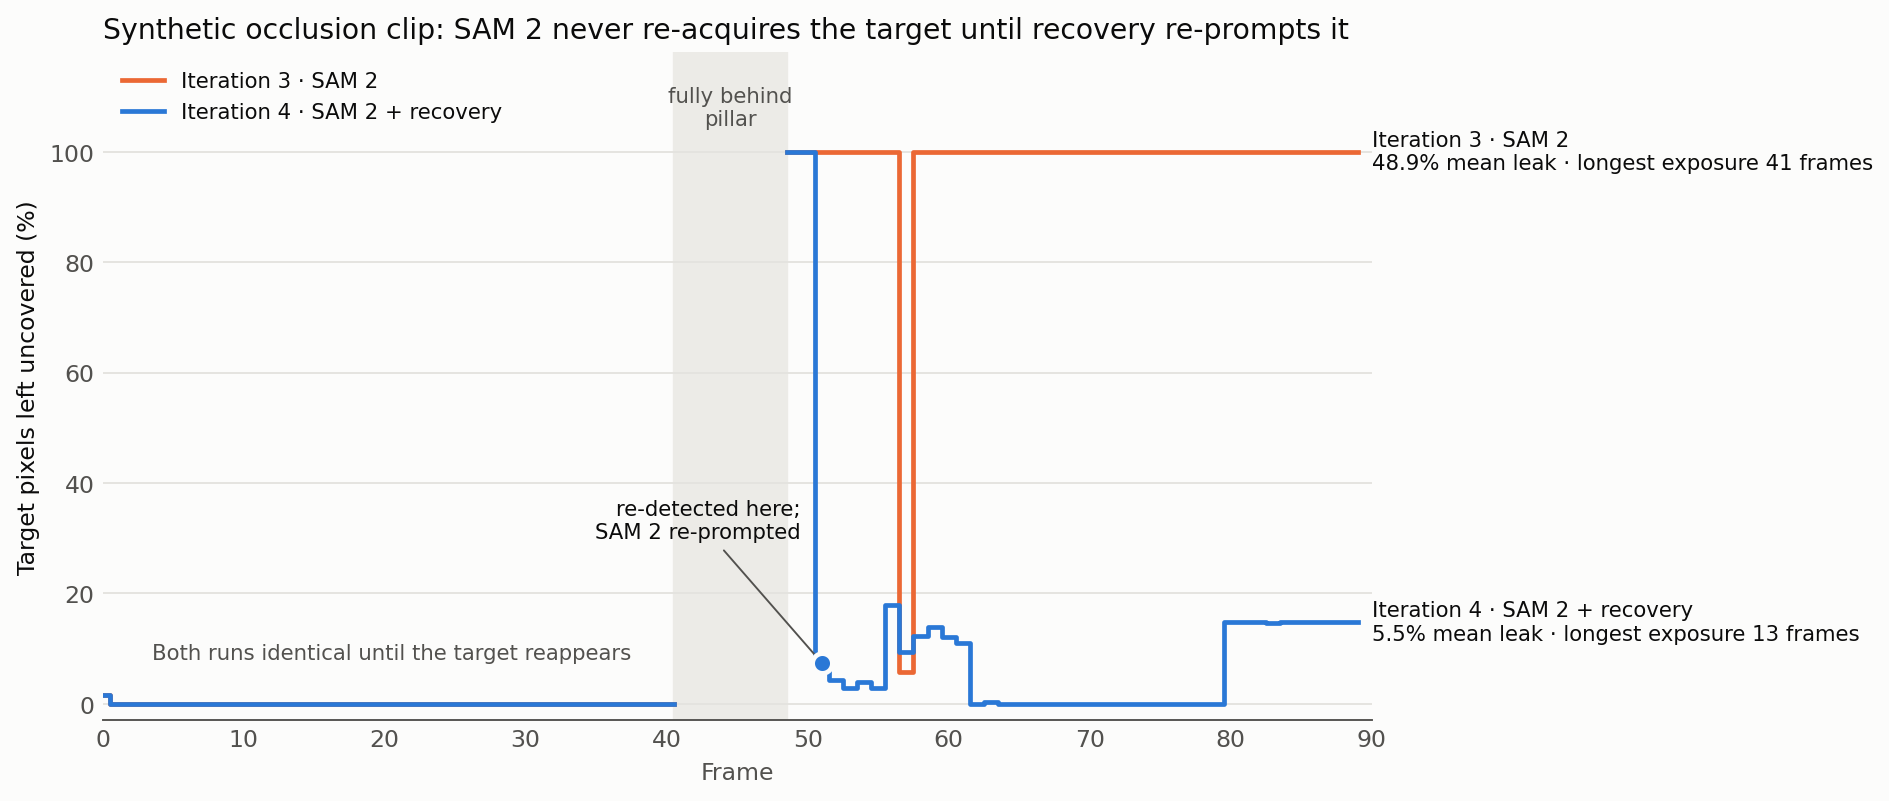
\includegraphics[width=0.92\linewidth]{figures/occlusion-timeline.png}
\caption{Synthetic pillar clip at 5-pixel slack. Both runs are identical until the target comes back
out, and recovery re-detects it at frame 51.}
\label{fig:occlusion}
\end{figure}

\begin{table}[h]
\centering\small
\begin{tabular}{llcc}
\toprule
Dataset & Metric & Iteration 3 & Iteration 4 \\
\midrule
Synthetic occlusion & IoU & 0.452 & \textbf{0.847} \\
Synthetic occlusion & Uncovered target & 48.9\% & \textbf{5.9\%} \\
Synthetic occlusion & Frames flagged for review & 54\% & \textbf{12\%} \\
Synthetic, all 4 clips & IoU & 0.776 & \textbf{0.875} \\
DAVIS (12 objects) & IoU & 0.836 & 0.836 \\
Crosswalk & IoU & 0.779 & 0.779 \\
\bottomrule
\end{tabular}
\caption{Iteration 4. Synthetic rows average three prompt sizes. We reran both columns together,
and the Iteration 3 rerun gives a DAVIS IoU of 0.836 compared with 0.835 in the original run.}
\label{tab:iter4}
\end{table}

\textbf{Result.} On the occlusion clip, the uncovered share dropped from 48.9\% to 5.9\% and the
longest stretch of exposure went from 41 frames to 13--17 (Figure~\ref{fig:occlusion},
Table~\ref{tab:iter4}). There are some limits to what this shows.
\begin{itemize}
\item \textbf{No real-video gain yet.} SAM~2 never lost a DAVIS or crosswalk target for 2 or more
frames, so recovery never ran there. That shows the change doesn't cost anything when it isn't
needed, but not that it helps on real footage. That's why real occlusion clips are in our plan.
\item \textbf{More usable, but not strictly safer.} Before, a lost target meant the whole frame got
covered (0.09\% leak, with 53.9\% of the frame covered beyond the target). Now those frames get a
target-shaped mask instead (3.47\% leak, 13.6\% extra coverage).
\item \textbf{Partly visible targets still leak.} The template needs most of the target in view,
so the first few frames after the pillar stay exposed.
\item \textbf{Wrong-person risk.} A lookalike could get re-detected. Rejecting ambiguous matches
helps, and recovered frames are flagged for review.
\end{itemize}

\subsection{Iteration 5: removing the target instead of covering it}

A black or blurred patch hides a person, but it also makes it obvious something was cut out, and a
big patch can ruin the shot. So we wanted to see if we could remove the target completely and show
the background behind it. This iteration reuses our selection and tracking and swaps the cover in
stage 4 for background reconstruction (Figure~\ref{fig:removal-pipeline}).

\begin{figure}[h]
\centering
\begin{tikzpicture}[
  font=\footnotesize, >={Stealth[length=4pt]},
  box/.style={draw, rounded corners=2pt, align=center, inner sep=3pt, minimum height=9mm},
  built/.style={box, line width=0.7pt, fill=blue!6, text width=24mm},
  flow/.style={->, line width=0.6pt},
  node distance=6mm,
]
\node[built] (a) {\textbf{Text prompt}\\Grounding DINO};
\node[built, right=of a] (b) {\textbf{Track}\\SAM 2.1 Base+};
\node[built, right=of b] (c) {\textbf{Align frames}\\ORB + RANSAC};
\node[built, right=of c] (d) {\textbf{Fill}\\masked temporal median};
\node[built, right=of d] (e) {\textbf{Fallback}\\Telea inpainting};
\draw[flow] (a) -- (b); \draw[flow] (b) -- (c); \draw[flow] (c) -- (d); \draw[flow] (d) -- (e);
\end{tikzpicture}
\caption{The removal pipeline.}
\label{fig:removal-pipeline}
\end{figure}

\textbf{Change.} The background behind a moving person is usually visible in some other frame, once
they've walked past. For each frame, we match ORB features \cite{orb} outside the target masks to
other frames in the shot, fit a homography with RANSAC \cite{ransac}, and warp those frames into
place. Each hidden pixel then takes the median of the frames where it's visible, using at least two
of them. Pixels that are never visible fall back to single-frame Telea inpainting \cite{telea}. We
don't train any model or use a generative video model, and pixels outside the expanded mask never
change.

\textbf{Evaluation.} We compared three ways of filling the same masks on 10 cases of 36 frames each.
Nine are synthetic (stationary, panning, and a hole that's never uncovered, with three seeds each).
The tenth is a real crosswalk clip with an artificial moving hole, scored against the held-out
pixels. These numbers measure reconstruction rather than tracking, so they can't be compared with
the IoU tables above.

\begin{table}[h]
\centering\small
\begin{tabular}{lccc}
\toprule
Mean RGB error in the mask (0--255) & Single frame & Unaligned median & Aligned median \\
\midrule
Stationary background & 27.80 & \textbf{0.00} & 0.02 \\
Panning camera & 27.95 & 32.29 & \textbf{0.82} \\
Background never visible & 27.95 & 27.95 & 27.95 \\
Real crosswalk + artificial hole & 44.08 & 25.91 & \textbf{17.74} \\
\bottomrule
\end{tabular}
\caption{Reconstruction error, where lower is better. Synthetic rows average three seeds, and the
crosswalk row is one sequence.}
\label{tab:removal}
\end{table}

\begin{figure}[h]
\centering
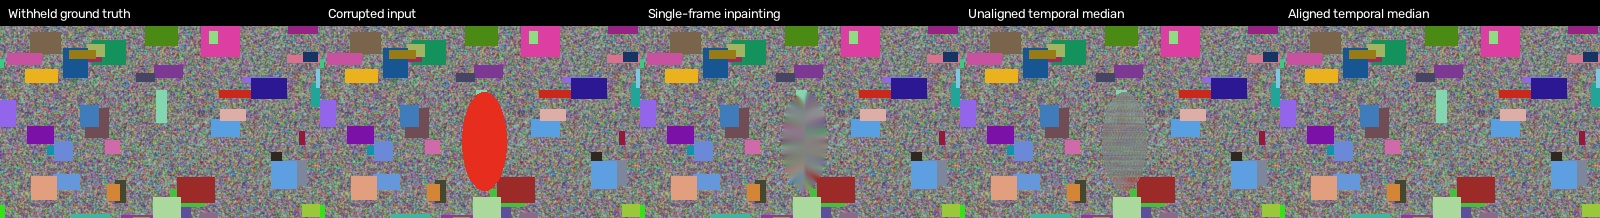
\includegraphics[width=\linewidth]{figures/removal-camera-pan.jpg}
\caption{Synthetic camera pan. From left to right are the withheld ground truth, the input with the
target, single-frame inpainting, the unaligned median, and the aligned median.}
\label{fig:pan}
\end{figure}

\textbf{Result.} Borrowing from other frames works well when the camera is still
(Table~\ref{tab:removal}). Once the camera pans, unaligned copying is actually worse than not
borrowing at all (32.29 vs.\ 27.95), and alignment fixes almost all of that (Figure~\ref{fig:pan}).
On the real crosswalk, alignment cut the error by 60\% compared with single-frame filling
(Figure~\ref{fig:removal}). When the background is never visible, none of the temporal methods
help, and the method correctly reports that no frame could see those pixels. One thing that didn't
go our way is that on the crosswalk, the aligned version flickered slightly more from frame to frame
than the unaligned one (temporal residual 12.34 vs.\ 11.70). That tells us source frames need to be
picked more consistently over time.

\begin{figure}[h]
\centering
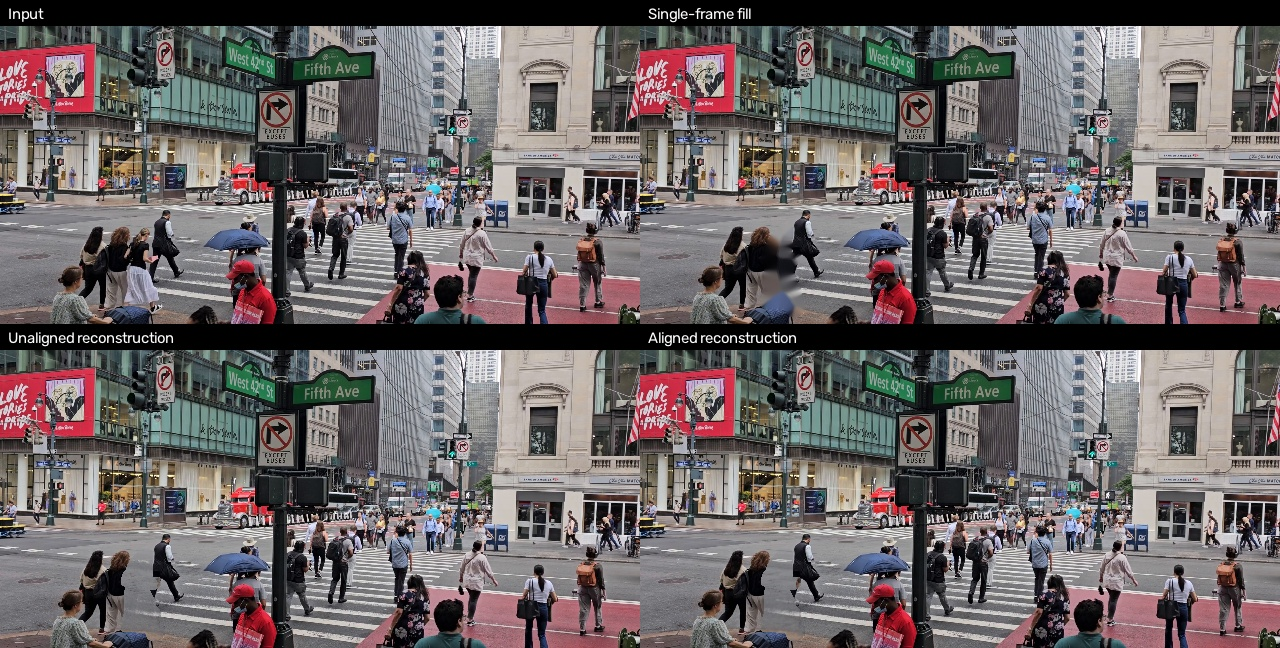
\includegraphics[width=0.92\linewidth]{figures/removal-crosswalk.jpg}
\caption{The proposal's crosswalk target removed using the text prompt ``woman wearing a white
skirt''. Single-frame filling smears, while aligned reconstruction recovers the crosswalk behind
her. Other moving pedestrians can still leave ghosts.}
\label{fig:removal}
\end{figure}

\textbf{Speed and model choice.} The first version was slow, so we profiled it. Only computing the
final method, using 8 source frames instead of 17, and turning on OpenCV's parallel loops took the
reconstruction step from 93.8\,s to 20.7\,s on the same test clip (4.5$\times$ faster), while error
went from 17.74 to 18.53. For tracking, we compared SAM~2.1 sizes on 31 crosswalk frames. Tiny was
the fastest (67\,s), but its masks spread onto nearby pedestrians (IoU 0.552). Base+ with half
precision took 119\,s at IoU 0.760, so we went with that. A full 150-frame Tiny run showed the same
failure (IoU around 0.38).

\textbf{How this connects to occlusion recovery.} Removal makes tracking mistakes a lot more
noticeable. With a cover, a missed frame leaks part of the target. With removal, a missed frame
makes the person suddenly pop back into a scene they were erased from, and their pixels can also
leak into the background used for other frames. So Iteration~4's re-detection matters even more
here. Text selection also just picks the highest-scoring box (0.820 for the skirt prompt and 0.919
for a dog clip), so someone still has to check the preview.

\subsection{Selection and review}
\label{sec:selection}

\textbf{Does the selection shape matter?} In the proposal, the outline did no better than a box on
the synthetic clips, and we said we'd need crowded real frames to really test it. We ran that test
on the six labeled crosswalk frames with three prompt sizes and three initialization methods, for
54 segmentations total. Each method got the same frame and slack.

\begin{figure}[h]
\centering
% One unchanged row from the saved comparison: frame 30, 9-pixel slack.
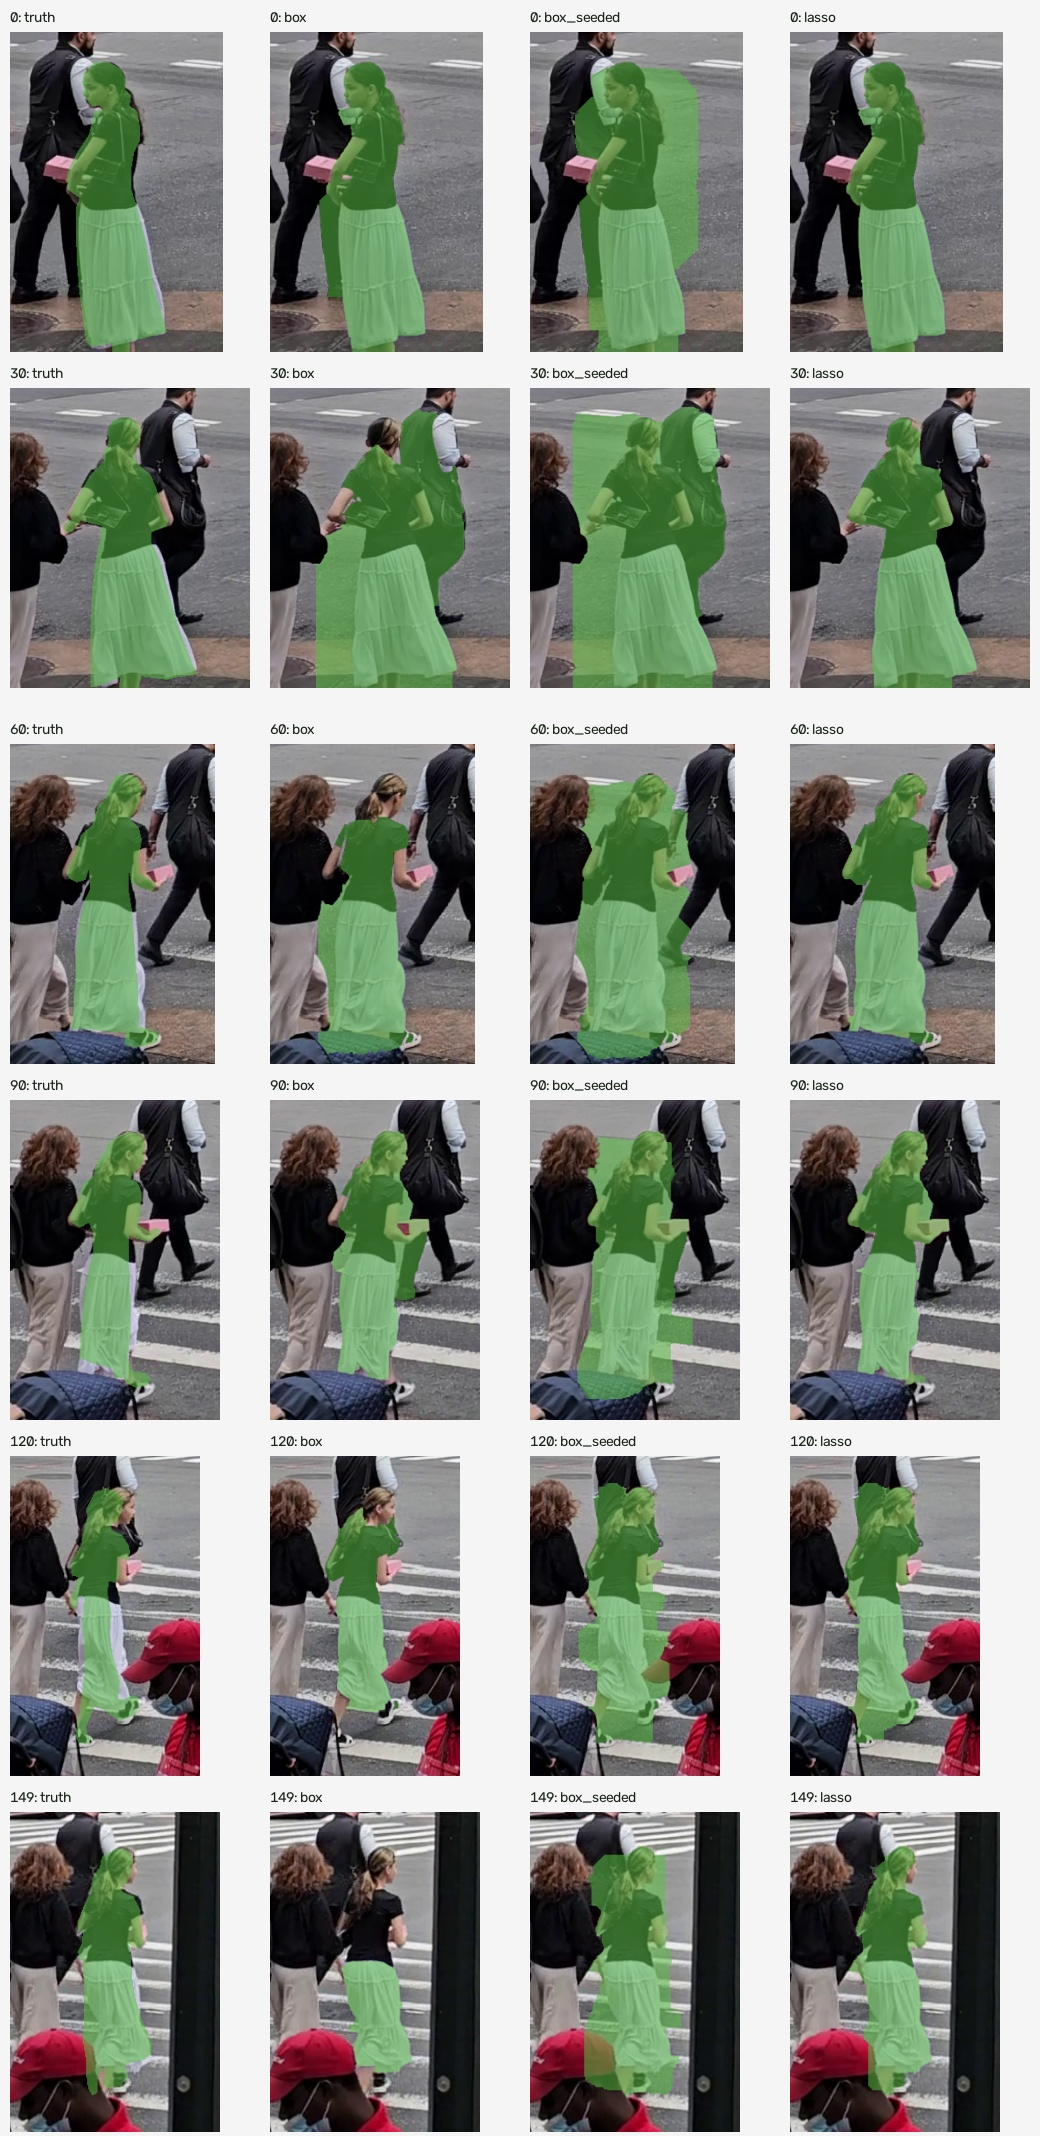
\includegraphics[width=0.9\linewidth,trim=0 1420 0 356,clip]{figures/prompt-ablation.jpg}
\caption{Crosswalk frame 30, showing the label, the box, the box with outline-style seeds, and the
outline. Green is the resulting mask, and the box picks up the person next to the target.}
\label{fig:prompt}
\end{figure}

\begin{table}[h]
\centering\small
\begin{tabular}{lccc}
\toprule
Initialization & IoU & Missed target & Extra frame area \\
\midrule
Original box & 0.620 & 14.92\% & 0.34\% \\
Box with outline-style seeds & 0.537 & 0.06\% & 0.77\% \\
Outline & 0.806 & 0.53\% & 0.24\% \\
\bottomrule
\end{tabular}
\caption{Initialization on six crosswalk frames, three prompt sizes each.}
\label{tab:prompt}
\end{table}

This backs up what we guessed in the proposal (Figure~\ref{fig:prompt}, Table~\ref{tab:prompt}).
In a crowd, a rectangle around one person picks up parts of the people next to them, and the
outline avoids that. The seeded box missed the fewest pixels, but only because it also covered more
background. We kept the outline as the default and the box as a quick option. Six frames of one
person is a small sample, and the prompts came from the labels rather than real users drawing them.

\textbf{Review app.} Users preview the mask before exporting (Figure~\ref{fig:preview}). Actually
using the app turned up a handful of bugs, which we fixed.
\begin{itemize}
\item Drawing right after a fast seek could use the old frame. Now a drawing only counts once the
displayed frame matches the selected one.
\item Focusing the canvas could scroll it mid-drawing. Now it focuses without scrolling, and we
test that coordinates stay lined up.
\item A target that left the scene kept getting tracked. We added an explicit end-target action.
\item Saved outlines depended on image files that might be missing. Now the polygon coordinates are
stored in the replay file.
\item A new selection could show an old preview. Now previews reset after edits and stale responses
get dropped.
\end{itemize}
All 26 local tests pass, including the optional model tests. Iteration~4 adds a regression test that
requires re-detecting the target after the pillar.

\begin{figure}[h]
\centering
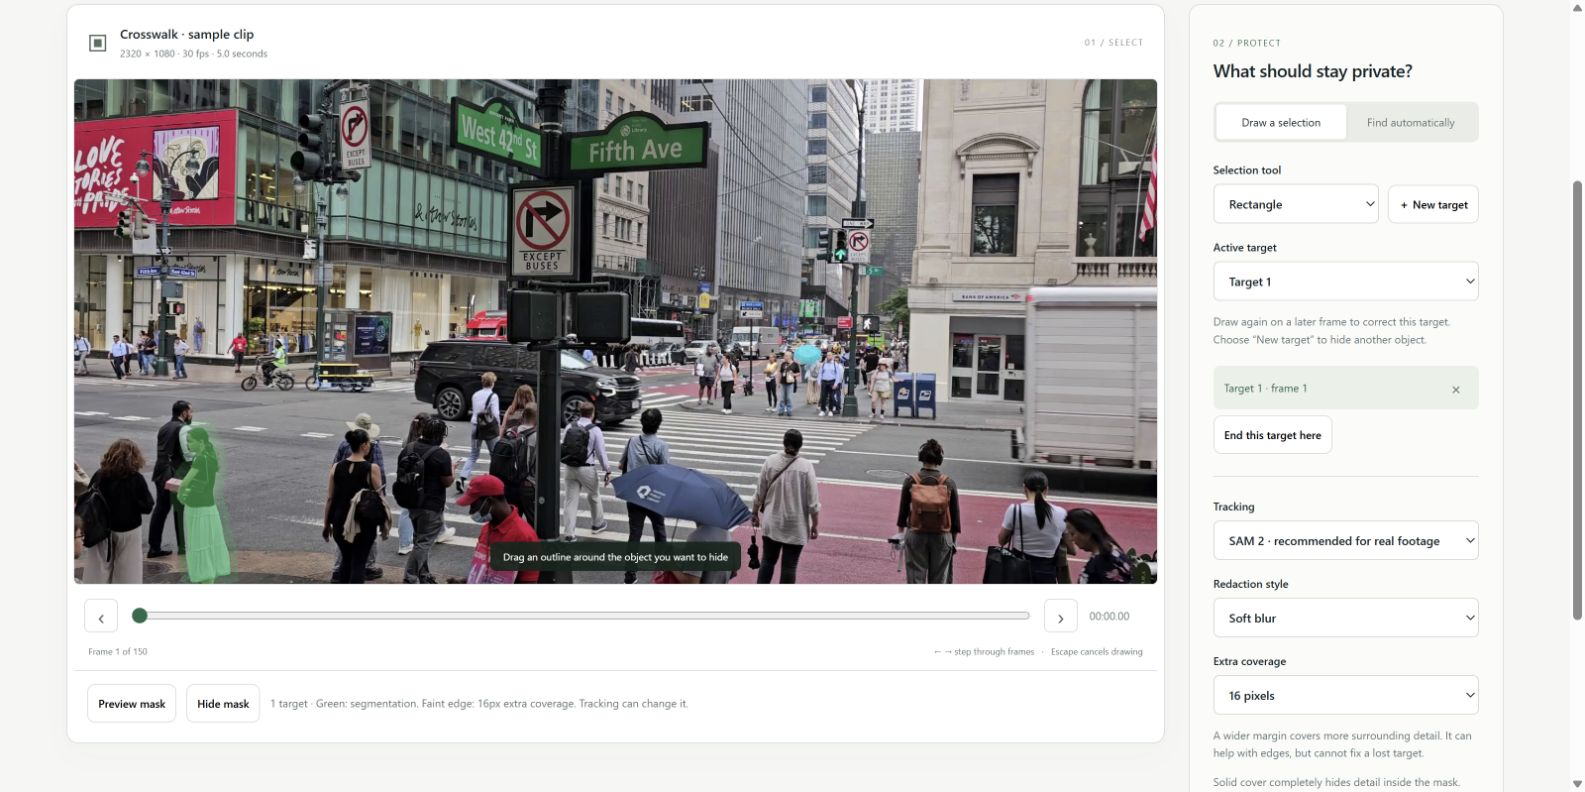
\includegraphics[width=0.6\linewidth]{figures/segmentation-preview.jpg}
\caption{The review app previewing a SAM 2 mask with a 16-pixel margin. Green is the selected
person.}
\label{fig:preview}
\end{figure}
